\documentclass{article}
\usepackage[utf8]{inputenc} % allow utf-8 input
\usepackage[T1]{fontenc}    % use 8-bit T1 fonts
\usepackage{hyperref}       % hyperlinks
\usepackage{url}            % simple URL typesetting
\usepackage{booktabs}       % professional-quality tables
\usepackage{amsfonts}       % blackboard math symbols
\usepackage{nicefrac}       % compact symbols for 1/2, etc.
\usepackage{microtype}      % microtypography

\usepackage[english]{babel}
\usepackage{blindtext}
\usepackage{bm}
\usepackage{index}
\usepackage[utf8]{inputenc}
\usepackage{graphicx}
\graphicspath{ {./} }
\usepackage{amsmath}
\usepackage{amssymb}
\usepackage{listings}
\usepackage{color}
\usepackage{siunitx}
\usepackage{longtable}

\definecolor{dkgreen}{rgb}{0,0.6,0}
\definecolor{gray}{rgb}{0.5,0.5,0.5}
\definecolor{mauve}{rgb}{0.58,0,0.82}

\lstset{frame=tb,
  language=Python,
  aboveskip=3mm,
  belowskip=3mm,
  showstringspaces=false,
  columns=flexible,
  basicstyle={\small\ttfamily},
  numbers=none,
  numberstyle=\tiny\color{gray},
  keywordstyle=\color{blue},
  commentstyle=\color{dkgreen},
  stringstyle=\color{mauve},
  breaklines=true,
  breakatwhitespace=true,
  tabsize=3
}
%% ========New command added by Han Liu===========================
\renewcommand{\vec}[1]{\boldsymbol{#1}}
\newenvironment{qparts}{\begin{enumerate}[1.]}{\end{enumerate}}
\usepackage{amsmath,textcomp,amssymb,geometry,graphicx,enumerate}
\usepackage{subcaption}
\usepackage[figurename=Fig.,labelfont=bf,labelsep=period]{caption}
\usepackage[capitalise]{cleveref}

\begin{document}
\title{EECS289A Introduction to Machine Learning,  Project T Final - Quiz Questions}
\author{%
  \ Han Liu, \ Peng Tan, \ Dilu Xu, \ Jinyan Zhao \\
  Department of Civil Engineering\\
  Universitu of California, Berkeley\\
  Berkeley, CA 94704 \\
  \texttt{\{han\_liu, tanpeng, diluxu, jinyan\_zhao\}@berkeley.edu} \\
}
\maketitle

\section{Elastic Net (HL)}
In class we discussed two types of regularization, $l_1$ and $l_2$. Both are useful, and sometimes it is helpful combine them, giving the objective function below (\textbf{in this problem we have excluded} $w_0$ \textbf{for simplicity}):
\begin{equation}
F(\vec{w}) = \frac{1}{2}\sum^n_{j=1}(y^{(j)}-\sum^d_{i=1}\vec{w}_i\vec{x}_i^{(j)})^2+\alpha\sum^d_{i=1}|\vec{w}_i|+\frac{\lambda}{2}+\sum^d_{i=1}\vec{w}_i^2
\end{equation}
Here, $(\vec{x}^{(j)},y^{(j)})$ is j-th example in the training data, w is a d dimensional weight vector, $\lambda$ is a regularization parameter for the $l_2$ norm of w, and $\alpha$ is a regularization parameter for the $l_1$ norm of w. This approach is called the Elastic Net, and you can see that it is a generalization of Ridge and Lasso regression: It reverts to Lasso when $\lambda = 0$, and it reverts to Ridge when $\alpha = 0$. In this question, we are going to derive the coordinate descent (CD) update rule for this objective.

Let g, h, c be real constants, and consider the function of x
\begin{equation}
f_1(x) = c+gx+\frac{1}{2}hx^2
\end{equation}
\begin{qparts}
\item {[}4 points{]} 
What is the $x^*$ that minimizes $f_1(x)$? (i.e. calculate $x^*=\arg\min f_1(x)$)\\
\underline{\textbf{Answer:}}\\
Take the gradient of $f_1(x)$ and set it to 0.
\begin{alignat}{2}
g+hx&=0 \\
x^*&=-\frac{g}{h}
\end{alignat}   

Let $\alpha$ be an additional real constant, and consider another function of x
\begin{equation}
f_2(x) = c+gx+\frac{1}{2}hx^2+\alpha|x|(h>0, \alpha>0)
\end{equation}
This is a piecewise function, composed of two quadratic functions:
\begin{equation}
f_2^-(x) = c+gx+\frac{1}{2}hx^2-\alpha x
\end{equation}
and
\begin{equation}
f_2^+(x) = c+gx+\frac{1}{2}hx^2+\alpha x
\end{equation}
Let $\tilde{x}^-=\arg\min_{x\in\mathbb{R}}f_2^-(x)$ and $\tilde{x}^+=\arg\min_{x\in\mathbb{R}}f_2^+(x)$.\\
(\textbf{Note:} The argmin is taken over $(-\infty, +\infty)$ here.
\\

\item {[}6 points{]} 
What are $\tilde{x}^+$ and $\tilde{x}^+$? Show that $\tilde{x}^-\geq\tilde{x}^+$. \\
\underline{\textbf{Answer:}}\\
Using the answer from part 1), we get $\tilde{x}^+=-\frac{g+\alpha}{h}$ and $\tilde{x}^-=-\frac{g-\alpha}{h}$. Since $\tilde{x}^--\tilde{x}^+=\frac{2\alpha}{h}\geq 0$, we have $\tilde{x}^-\geq\tilde{x}^+$.


\item {[}12 points{]} 
Draw a picture of $f_2(x)$ in each of the three cases below:
\begin{enumerate}[(a)]
\item $\tilde{x}^->0$, $\tilde{x}^+>0$
\item $\tilde{x}^-<0$, $\tilde{x}^+<0$
\item $\tilde{x}^->0$, $\tilde{x}^+<0$
\end{enumerate}
For each case, mark the minimum as either 0, $\tilde{x}^-$, or $\tilde{x}^+$. (You do not need to draw perfect curves, just get the rough shape and the relative locations of the minima to the x-axis)\\
\underline{\textbf{Answer:}}\\
\cref{fig:hl1} gives the example picture of three cases. To understand the answer, note the following
\begin{figure*}[!htb]
    \centering
    \begin{subfigure}[t]{0.31\textwidth}
        \centering
        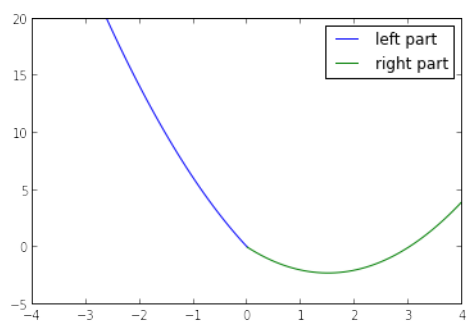
\includegraphics[height=1.3in]{fig/fig-han-1.PNG}
        \caption{$\tilde{x}^->0$, $\tilde{x}^+>0$, the minima is at $\tilde{x}^+$.}
    \end{subfigure}%
    ~
    \begin{subfigure}[t]{0.31\textwidth}
        \centering
        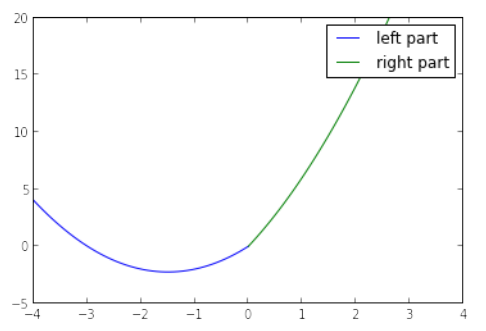
\includegraphics[height=1.3in]{fig/fig-han-2.PNG}
        \caption{$\tilde{x}^-<0$, $\tilde{x}^+<0$, the minima is at $\tilde{x}^-$.}
    \end{subfigure}
    ~
    \begin{subfigure}[t]{0.31\textwidth}
        \centering
        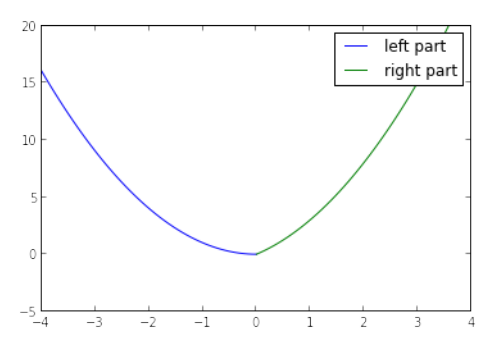
\includegraphics[height=1.3in]{fig/fig-han-3.PNG}
        \caption{$\tilde{x}^->0$, $\tilde{x}^+<0$, the minima is at 0.}
    \end{subfigure}
    \caption{Example picture of three cases.}
    \label{fig:hl1} 
\end{figure*}


\item {[}12 points{]} 
\end{qparts}
\end{document}